\chapter{Related Work on Solutions to Identified Problems}
\label{chap:prev_research}

In this chapter, we discuss some of the solutions that have been proposed or used by the different researchers. The solutions discussed here are limited in the scope of the problems identified in the last chapter. It is important to note that there have been numerous papers studying the different treebanks in UD, and the set of problems encountered while changing the annotation from the guidelines for UDv1 to UDv2. While such research is helpful in pointing out cases where the annotating teams had difficulties during the conversion procedure, we do not discuss those references here, unless needed.

Before proceeding further, it is imperative to understand a subtle difference between error detection and inconsistency detection. If the errors are consistent in their distribution across the data, an inconsistency detection tool would fail in the discovery of such errors. In such case, the non erroneous part of the annotation would be the inconsistency and might be flagged as a false negative, provided the tool is biased towards the erroneous annotation. Any tool that tries to discover inconsistencies need not find such consistent error patterns. This is the major difference between error detection and inconsistency detection. Error mining methods are primarily based on detecting deviations from a standard clean reference (usually gold or platinum standard), and should be able to provide an analysis of the error patterns regardless of whether or not the error is present consistently. In this chapter, we use error mining and error detection interchangeably.

The rest of the chapter is organised as follows. We first discuss existing literature on inconsistency detection in Section \ref{sec:inconsistency-detection}, and the relevance of the literature to the problem identified in Section \ref{sec:harmony} on Annotation Consistency in Different Treebanks. We then focus on the literature relevant to error detection in Section \ref{sec:error-mining}.

\section{Annotation Consistency across Treebanks}
\label{sec:inconsistency-detection}

Owing to different annotation schemes for the different treebanks of a given language, there is no standard evaluation metric to compare the consistency of treebanks' annotation to each other to the best of our knowledge. 

One of the most commonly used approaches to find the inconsistencies in the annotation is to train a high quality parser/tagger model on a given training data, and evaluating the cases where the prediction from the trained model differs from the annotation of the test data. This approach can also be extended by bootstrapping different trained models, with the majority consensus being compared against the available annotation. While this approach can point to individual inconsistencies, it does not say anything about the errors in the treebank. Furthermore, the different treebanks of the same language can have different annotation inconsistencies with the errors being consistent in their presence throughout. Additionally, the consistent errors in the different treebanks can be vastly different from each other as well.

To ascertain annotation quality of one or more treebanks, both inconsistency detection and error detection should be used. In case of individual treebanks, UD website\footnote{\url{universaldependencies.org}} shows against each treebank a metric score that is an approximation of the quality of the treebank. The metric is calculated heuristically\footnote{For more details on the associated heuristics, refer to \url{https://github.com/UniversalDependencies/tools/blob/master/evaluate_treebank.pl}}, depending on multiple factors like the number of genres present in the treebank, the score as provided by official UD validator\footnote{refer to \url{https://github.com/UniversalDependencies/tools/blob/master/validate.py}}, among others. When it comes to comparing annotation quality among multiple treebanks, there exist no metrics or tools to the best of our knowledge. However, some techniques have been used more often than others for such comparisons.

\subsection{Consistency in POS Annotation}
\label{ssec:inconsistency-detection-pos}

\cite{dickinson03a, dickinson03b} are the most well known pieces of work in detecting inconsistency in POS annotation, essentially forming the base of majority of inconsistency detection. The work focuses on finding a n-gram of tokens in the corpus that occurs in the same context (referred to as a variation nucleus) such that the different occurrences of the variation nucleus are annotated differently. Originally coined for continuous annotation\footnote{The annotation of the current token is based on the annotation of a contiguous token in word order. Discontinuous annotation implies the annotation of current token is dependent on another token that might not be contiguous in the word order, as in the case of dependency parsing.}, the method was eventually adapted to look for inconsistencies in discontinuous annotation as well \citep{dickinson05}.

\cite{korean} compare the POS annotation consistency for different treebanks in \verb|ko| by using the relative frequency of the individual POS tags. The authors also briefly mention the cause of the variation in distribution of the individual POS tags. While such analysis is slightly helpful in terms of drawing a comparison, it does not consider the interaction of different POS tags with each other. To illustrate such interactions, a n-gram based approach might be utilised. Even so, absence of \verb|SCONJ| tag in one treebank prevents the analysis with respect to other treebanks.

\subsection{Consistency in Dependency Annotation}
\label{ssec:inconsistency-detection-deprel}

The original method of using variation nuclei for continuous annotation as proposed by \cite{dickinson03a, dickinson03b} was extended for discontinuous annotation in \cite{dickinson05}, as mentioned earlier. By extending the method to discontinuous annotations, \citeauthor{dickinson05} were able to look at more patterns in TIGER corpus. Moreover, this meant that instead of looking at plain POS tags and identifying the variations therein, the words could now be looked at in order to generalize the context.

\cite{alonso2016universal} compared the treebanks for \verb|es| in UDv1.3 \citep{UDv1.3}. They assess the similarity of the different treebanks using dependency parsing. A high-efficiency parser was trained on one of the treebanks, and then tested on another. The idea was to notice the drop in LAS scores, and if the difference in scores was more than what was intuitive, the treebanks were marked as not similar enough. The same technique of evaluating the different treebanks for \verb|ru| against each other was also used in \cite{RussianTreebanks}. In their work spanning the different \verb|ru| treebanks in UD, \citeauthor{RussianTreebanks} also point out problems with individual treebanks. The problems pointed out therein can be used as a starting point to scout for patterns that are present across the different treebanks for the language. 

\cite{CLAS} proposed an evaluation metric called CLAS (Content-based LAS) score that disregard the punctuation and other functional nodes, evaluating LAS based on content words only. The change of evaluation metric from LAS to CLAS was meant as a way to give equal treatment to the languages with weak morphology and languages with strong morphology. For example, a single inconsistency in \verb|fi| will affect the parsing score more than a single inconsistency in \verb|en| owing to the differences in the extent of morphology used by the languages. The metric was evaluated as a secondary measure in CoNLL 2017 Shared Task \citep{CLAS_test}. The primary metric for the Shared Task was macro-averaged LAS score for the different languages. It was reported that the there is no significant performance difference in parser performances when the evaluation metric was changed from macro-averaged LAS score to CLAS score.

An important point to note here is that the metrics LAS and CLAS are associated with the performance of parsers. The metric scores would be lower in case even when the parser is able to parse the data better than the manual annotation. The two metrics (and also unlabelled attached score or UAS) therefore cannot be relied upon for detection of the inconsistencies.

\cite{korean} compare the dependency annotation consistency among different treebanks in \verb|ko| by again focusing on the relative frequency of the dependency labels, offering reasons for the variation in distribution of the individual label. A dependency label is determined by the choice of the parent label as well, and thus the method of \citeauthor{korean} is of little help in flagging any inconsistencies.

\subsection{LISCA}
\label{ssec:lisca_soln}

\cite{lisca} used an unsupervised algorithm which attempts to find the inconsistencies in dependency annotation by building a statistical model on the data from a given reference corpus (ideally, a gold standard). This algorithm, called LISCA, creates a language model for the given dependency arcs, learning for each arc its probability of occurrence based on a subset of local and global attributes associated with the arc. The eventually created language model can then be used to rank the dependency arcs in another parsed corpus by their probability of occurrence. Figure \ref{fig:lisca_stats} shows graphically some of the features used by LISCA to calculate score for an arc.

\begin{figure}[H]
    \centering
    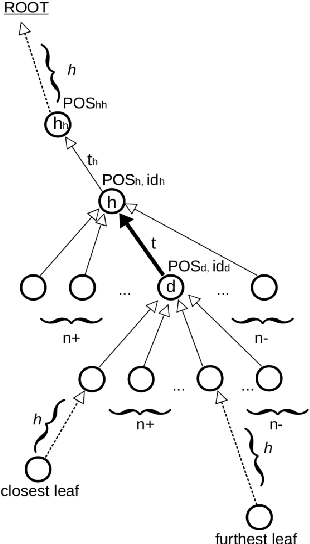
\includegraphics[scale=0.5]{img/lisca_stats.png}
    \caption[Features Used by LISCA to Calculate Plausibility Score for an Arc]{Features Used by LISCA to Calculate Plausibility Score for an Arc (marked in bold). Figure borrowed from \cite{alzetta2017dangerous}}
    \label{fig:lisca_stats}
\end{figure}

LISCA was used to identify the errors in newspaper section of Italian UD Treebank in \cite{alzetta2017dangerous}. In their work, they narrow the search space for the errors by binning the arcs according to the scores into 10 bins of equal size and an extra bin to include the extra cases. The bins were then manually inspected for errors, while concentrating on the last two (and the extra) bins containing the arcs with lowest scores. Analysing the data, 36\% of the arcs in the low ranking bins consisted of random errors, while the remaining ones were found to be systemic and recurrent errors (even in treebanks of different languages).

While the algorithm mentioned above successfully points out the arcs that are inconsistent in their annotation in the different datasets, it is sensitive to the genre of the data. The authors note that the data should ideally belong to the same register/genre for the algorithm to function at its best. While this is problematic because in some treebanks it is not possible to separate the data from different genres, there is also a possibility of unavailability of enough data in a particular genre (i.e. a single genre contributing in a very small manner to the size of the treebank).

Added to these difficulties is the difficulty of training the algorithm. The algorithm essentially needs to be trained on a gold standard data, from which it builds a statistical model that is used to generate the probability scores of a dependency arc. In case of languages with no high-quality parsers available or for low-resource languages, this poses a cold-start problem where we do not have the data to train the algorithm, and so the algorithm cannot be used at all.

We tried solving this problem of cold-start by using the method of \(k\)-fold cross validation (with varying values of \(k\)) in training the algorithm. We discuss the experiment in more detail in Chapter \ref{chap:lisca}.

\section{Error Mining Methods}
\label{sec:error-mining}

Error mining in treebanks can be done in multiple ways. There is a possibility of using hand-written rules, and scouting for the patterns in the relevant treebank. This manual approach works well for finding error typologies that are known beforehand. The other approach is to combine the statistical approach, with the manually defined rules \citep{ambati}. This method is referred to as heuristics-based search since it identifies a lot of patterns, which can then be used to look for errors in the data (in some cases, this can be done automatically). The last approach is automatic scouting for error patterns within the scope of the treebank, also known as automatic error mining.

\subsection{Error Mining Based on n-gram Approach}

\cite{boyd} first introduced the idea of error mining methods in dependency treebanks using variation nuclei, expanding on the idea of using n-grams based variation nuclei for discontinuous annotations from \cite{dickinson05}. This is often referred to as the first automatic error mining method in dependency treebanks.

\cite{de2017assessing} extended and evaluated the method proposed by \citeauthor{boyd}, in context of UD Treebanks for three languages (\verb|en|, \verb|fi|, \verb|fr|). The authors further extended the method to use word lemmas instead of simply using word forms, and also evaluate on the automatically annotated treebanks to identify more inconsistencies. The first extension of using lemmas works well for languages that are not too morphologically-rich (\verb|en|, \verb|fr|), but fails otherwise. The second extension is done at the cost of a drop in precision, but without a significant gain in recall.

The method proposed by \citeauthor{boyd} has an inherent problem instance of data sparseness. \cite{kook} implemented an algorithm based on n-grams and suspicion sharing across the n-grams by extending the methods of \cite{sagot} and \cite{noord}. Their approach however, relies on classifying each sentence within the results of a parsed corpus as a parsable or unparsable sentence. This classification of individual sentence needs to be done manually, and is therefore not optimal for large treebanks.

\newpage